\section{Methodology}

This section details the theoretical and practical framework developed to address dynamic pricing under the influence of non-human actors. We begin by formalizing the problem environment and the nature of the actors. We then derive the \textit{Cost of Information} (COI) theorem, proving the erosion of pricing power in the limit of agent saturation. Following this, we outline our generative contamination strategy using GOFAI-driven distinguishability and transition probability learning. Finally, we formulate the robust control problem as a Stackelberg game solved via Distributionally Robust Reinforcement Learning (DR-RL) with constructed ambiguity sets.

\subsection{Problem Formalization}

We define a commercial environment where the platform interacts with a stream of sessions. Each session belongs to the set of all sessions. Each session is generated by an actor belonging to a latent class, either Human (H) or Agent (A).

Each session produces a trajectory of observable events. An event is a tuple containing:
the action taken (e.g., view item, add to cart),
the target item index,
and the continuous timestamp.

The platform does not directly observe the true underlying demand function. Instead, it observes a behavioral proxy, which is a composite signal derived from the mixture of actor types. We define the demand proxy for product i at epoch t as a weighted aggregation of events: for each session in a time period, we sum up all the events where a specific product was interacted with, and we weight those events by how strong a signal they provide about willingness to pay. For example, adding an item to a cart is a stronger signal than just viewing it.

In the current engine implementation, we use the normalized variant of this proxy for each step: we scale the raw demand signal for each product to a percentage out of 100, distributing it proportionally across all products. This keeps the signal dense and directly usable in the simulator. The weights follow a fixed category-level ordering: cart actions have the highest weight, then dwell actions, then navigation, then filtering.

\subsubsection{Actor Types and Demand Curves}

We formalize the heterogeneity of actors by introducing a type space. An actor of class H or A is further parameterized by a type that determines their demand response function. This type is sampled from a distribution of possible demand curves. The total observed demand is a stochastic process governed by the mixture:

Total observed demand equals a combination of human demand (weighted by one minus the contamination ratio) and agent demand (weighted by the contamination ratio), plus some temporal market noise. The contamination parameter represents the proportion of agents in the system and ranges from 0 to 1.

\subsection{Cost of Information (COI) Framework}

The platform's pricing power comes from information asymmetry: users who express strong interest signals pay more than the base price. We quantify this markup as the \textit{Cost of Information} (COI), which represents the average premium extracted above marginal cost. COI measures the revenue at risk when information asymmetry collapses.

A top-level view in the current AI discourse is that sufficiently large productivity gains can induce vertical deflation through cost compression and supply expansion \parencite{rachitsky_marc_2026}. Our contribution is narrower and mechanism-level: even under long-run deflation, platform revenue still depends on short-run information costs to the user. We formalize that rent as the Cost of Information (COI) and study how agentic reconnaissance accelerates its erosion.

\textbf{Definition: Cost of Information.} The COI is defined as the difference between the expected price charged by the pricing policy and the minimum viable price (marginal cost). In other words, COI measures how much extra revenue the platform extracts on average by observing user behavior, beyond what it would get if everyone paid the rock-bottom price.

\begin{figure}[ht]
    \centering
    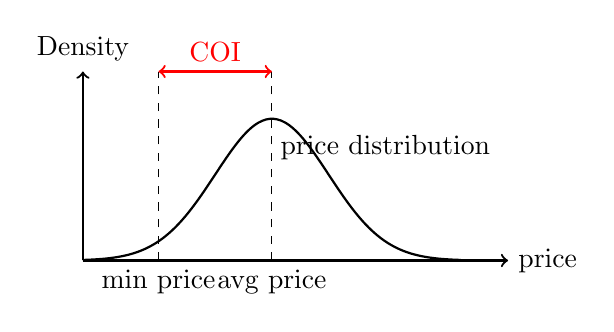
\begin{tikzpicture}[scale=1.2]
        % Define the Gaussian function: centered at 2
        \def\bellcurve(#1){1.5 * exp(-0.5*((#1-2)/0.6)^2)}

        % Draw the main axis
        \draw[->, thick] (0, 0) -- (4.5, 0) node[right] {price};
        \draw[->, thick] (0, 0) -- (0, 2) node[above] {Density};

        \draw[thick, smooth, samples=100] plot[domain=0:4] (\x, {\bellcurve(\x)});
        \node at (3.2, 1.2) {price distribution};

        % Define minimum price and average price
        \def\pmin{0.8}
        \def\mean{2}

        % Vertical lines
        \draw[dashed] (\pmin, 0) -- (\pmin, 2.0);
        \draw[dashed] (\mean, 0) -- (\mean, 2.0);

        % Labels on axis
        \node[below] at (\pmin, 0) {min price};
        \node[below] at (\mean, 0) {avg price};

        \draw[<->, thick, red] (\pmin, 2.0) -- (\mean, 2.0) node[midway, above] {COI};

    \end{tikzpicture}
    \caption{Illustration of the Cost of Information (COI). The COI is defined as the difference between the expected price realized by the policy and the minimum viable price.}
    \label{fig:coi_illustration}
\end{figure}

We now formally demonstrate that standard dynamic pricing mechanisms are not incentive-compatible with high-frequency agentic traffic. As the number of independent competitive agents querying the system grows, the platform's ability to sustain a COI vanishes.

A fundamental assumption for our claim lies in the alignment of the AI agent through its prompt which has been demonstrated by \textcite{fish_algorithmic_2025} to cause strong collusive behavior under linguistic nudges. This assumption can be generalized to the human user asking the agent to research products with a minimizing objective.

\textbf{Theorem: COI Erosion in the Limit.} Let N be the number of independent, utility-maximizing agents querying the platform. Let the minimum price be the lowest price offered to these agents. As N grows toward infinity, the Cost of Information converges to 0.

\textbf{Proof sketch.} Consider N independent agents querying the platform, each receiving a price sample drawn from the pricing policy's distribution bounded by a minimum and maximum price. A strategic agent conducting reconnaissance will select the minimum observed price.

The probability that the minimum price exceeds some threshold equals the probability that all sampled prices exceed that threshold. This can be written as a product: since the samples are independent, the chance that all N prices are above the threshold equals the chance that one price is above it, raised to the power N.

For any price above the minimum, there is always some positive probability of seeing a lower price. So the probability that one sample exceeds the threshold is less than 1. When we raise a number less than 1 to higher and higher powers (as N grows), it decays exponentially toward zero.

The expected minimum price can be written as the minimum price plus an integral that captures the tail probability. As N grows, this tail probability vanishes for all prices above the minimum, so the integral converges to zero. Therefore, as the number of agents increases, the expected minimum price approaches the floor price, and the Cost of Information (the difference between expected price and minimum price) vanishes.

This result proves that standard pricing policies fail to extract surplus in the presence of large-scale agentic search, necessitating a robust counter-mechanism.

\subsection{System Architecture: Hybrid Kappa-Lambda Architecture}

In order for our research to have grounding in interactions we built a robust e-commerce web-platform. We initially conducted a survey of the leading platforms of airlines and hotel booking sites to identify the specific interface patterns that effectively manage complex travel data. Our analysis revealed a clear industry standard: while both sectors rely on tabbed service selection and left-sidebar filtering to streamline navigation, they diverge in result presentation: airlines utilize visual date-price bars and multi-step wizards to optimize for logistical transparency, whereas hotel platforms leverage image-led cards and scarcity triggers to drive emotional engagement and urgency. Our web framework defines a highly agnostic boilerplate which can be seeded with any data-modality with an easy-to-tailor pattern, which we leverage to define a hotel and airline mode. Both modes are then individually deployed via an environment level argument which adjusts the proxy routing with a custom middleware inside next.js to render only the desired mode. The purpose of this was to create a baseline adaptable to any use-case or desired commercial application.

The architecture of this platform begins with the deployed web-apps posting interaction data to our backend which processes them and stores each ingested interaction into a kafka cluster. This serves as our data reservoir tracking and associating each interaction with its session and importantly with which experiment it belongs to. Not only do we track the behavioral interactions, but our pricing provider micro-service, once called by the frontend reports the observed/queried price-product into kafka. This kafka cluster is subscribed to by our pipeline which is configured on a schedule in Airflow, with the possibility of manual trigger. The final stage of the pricing pipeline, submits computed dynamic pricing results into a redis database for quick updates which is then read by the pricing provider and displayed on the webapp. This is a very generic end-to-end mechanism which is applicable to a variety of different e-commerce tasks. We intentionally put emphasis on the development of this infrastructure to establish a reproducible framework for interaction and to minimize any noise.

\paragraph{Public Web Artifact} We transition the Kappa like architecture of the data collection to a Lambda architecture for actual learning in a surrogate environment. This allows us to move faster on data which is provided and helps us create a feedback loop for production deployment. To support further research in this intersection of fields we release P4P \footnote{\url{https://github.com/velocitatem/p4p}} as a public repository providing the interaction layer of the PHANTOM framework. This provides a configurable storefront which can be tailored to any commercial setting with a standardized session-level event tracking. We document the API adapters or what the framework expects in terms of schemas for pricing providers and log ingestion servicse. The repository is intended for controlled experimentation and method replication rather than production commerce deployment.

\subsubsection{DevOps Principles}

Reproducible results are key to quality research platforms, this is taken into mind when deploying and working with our research platform. From a deployment standpoint the platform can be deployed across a large variety of providers and can be run locally. When developing a new interaction modality apart from the ones that come out of the box, a simple template pattern can be followed. The middleware of the framework is designed to properly render the chosen modality from environmental variables, thus deployment of different or parallel version of the software can be easily parametrized.

\subsubsection{Online Dynamic Pricing}

In order to collect data from actors under correct conditions we replicate a naive and simple dynamic pricing algorithm which runs in the background during the experiments.

The dynamic pricing done is handled by a pipeline which computes a demand estimate on a per-product basis of a specific window of the data, defined by the period T which by default is 5 minutes. This dynamic pricing pipeline computes a demand estimate vector by a weighted sum of interactions for each product, it additionally computes a price elasticity vector in the same dimensions as our demand. The final features matrix contains two columns for each product: demand and elasticity.

The transformation that governs this dynamic pricing is a very simple surge-based pricing: for each product, if the estimated demand is high enough (above a surge threshold), we multiply the base price by a surge factor (typically 1.2). If demand is low enough (below a discount threshold), we multiply by a discount factor (typically 0.9). Otherwise, we keep the base price unchanged.

This piecewise function enables rapid price adjustment in response to observed demand without requiring complex elasticity estimation or historical calibration, allowing us to expose actors within our experiments to a system with a dynamic component of pricing.

\subsection{Experimental Design}

We start from a practical constraint: we do not have access to proprietary production data. Because of that, we design our own fictional platform that still represents how commercial platforms work in the real world. The design comes from a survey of hotel and airline websites, where we extracted common interface components and used them as a high-level template for dynamic pricing environments.

The interface is organized as a product catalog where each product belongs to a time-bounded price vector (for example, a daily pricing period). During each period we collect interaction data by instrumenting UI components and predefined action templates that are still customizable. This gives us control without losing realism.

Since users act with motivations, we define a pool of tasks (jobs to be done) and assign tasks randomly to participants. The task pool is stored as a structured table with fields for task ID, creation timestamp, task name, description, and definition of done. We formulate the tasks as compact jobs-to-be-done rather than as strict click scripts, because the target is to elicit realistic browsing and comparison behavior which can capture nuance of different people. In hotel mode the assigned tasks include \textit{Cheapest Room}, \textit{Cheapest Room w/ View}, \textit{MultiStep Cheapest Room}, \textit{The Digital Nomad (Executive)}, and \textit{The 3-Way Tradeoff (Desk + Quiet + Flexible)}. These prompts deliberately require critical thought in search, inspection of room details, comparison of amenities or images, return visits to the listing page, and a final booking decision which create a degree of cognitive load. In airline mode we use \textit{Last-Minute One-Way Flight}, where the actor must urgently travel to LAX from either SEA or JFK within the next 1--3 days, inspect at least a small set of candidate itineraries, and then book a reasonable earliest departure.

A representative task is to find the cheapest feasible catalog item under explicit constraints while removing strict financial limits so we avoid trivial optimization behavior. Participants are also randomly assigned to one experimental platform mode (hotel or airline). Once assigned, they are dropped into the experiment with an actor ID. Under each experiment ID, we can observe multiple sessions across time and gather long interaction traces for the same actor.

The human data collection involved 13 participants, all of whom provided explicit informed consent prior to their session. Participants had an average age of 21 years and were recruited from a university population. Alongside the 13 human sessions we ran 16 agent sessions of equivalent task scope, yielding 29 labeled trajectories in total (45\% human, 55\% agent). Each participant was assigned a single platform mode and a single task drawn from the pool, and completed the session independently without guidance on navigation or pricing strategy.

To evaluate quality and realism of the setup, we store both structured event logs and full interaction transcripts. This lets us combine quantitative analysis with transcript-level qualitative findings. The result is an isolated system where we can control the interaction process while preserving realistic behavior.

Operationally, goals and experiment runs are tracked in PostgreSQL. This data-acquisition phase is the first half of the methodology and is intentionally a disconnected component that feeds the later contributions. The second half uses collected behavioral traces to distinguish classes (agent vs human) with session-conditioned probability estimates, then injects those estimates into the pricing learner.

Our process follows three stages: (1) observe and vectorize behavioral interactions, (2) learn distinguishability to characterize human versus agent patterns, and (3) use the learned signal to train a defensive policy in a controlled dynamic-pricing simulator.

\begin{figure}[ht]
  \resizebox{\columnwidth}{!}{%
    \definecolor{mygreenfill}{RGB}{169, 234, 186}
\definecolor{mygreenborder}{RGB}{29, 145, 61}
\definecolor{mybluefill}{RGB}{204, 222, 255}
\definecolor{myblueborder}{RGB}{66, 106, 189}
\definecolor{mygray}{RGB}{150, 150, 150}



\begin{tikzpicture}[
    node distance=2cm,
    % Style for Green Nodes
    greenbox/.style={
        rectangle,
        draw=mygreenborder,
        fill=mygreenfill,
        line width=1.2pt,
        align=center,
        minimum height=1cm
    },
    % Style for Blue Nodes
    bluebox/.style={
        rectangle,
        draw=myblueborder,
        fill=mybluefill,
        line width=1.2pt,
        align=center,
        minimum height=1cm
    },
    % Style for Arrows
    myarrow/.style={
        ->,
        >={Stealth[length=3mm, width=2mm]},
        draw=black!80,
        line width=1.2pt,
        rounded corners=5pt
    },
    % Style for Background Dashed Circles
    dashedloop/.style={
        dashed,
        draw=mygray,
        line width=1pt
    }
]

    % --- Coordinate Layout ---
    % Defining a grid relative to the center

    % Left Loop (Green) Nodes
    \node[greenbox, minimum width=3.5cm] (commerce) at (-3.5, 2) {Commerce Experiment};
    \node[greenbox, minimum width=1.5cm] (raw) at (-6.5, 0) {Raw\\Logs};
    \node[greenbox, minimum width=1.5cm] (features) at (-4, -2.5) {Features};
    \node[greenbox, minimum width=2.5cm] (classification) at (-1, -0.5) {Classification\\Training A/H};

    % Right Loop (Blue) Nodes
    \node[bluebox, minimum width=2.5cm] (trainedpricing) at (3.2, 2) {Trained Pricing};
    \node[bluebox, minimum width=2.5cm] (policy) at (6.5, 0) {Trained Pricing\\Policy};
    \node[bluebox, minimum width=2.5cm] (rlgym) at (3.2, -2.2) {RL Gym\\Training};

    % --- Background Dashed Loops ---
    \begin{scope}[on background layer]
        % Left Loop Circle
        \draw[dashedloop] (-3.5, 0) ellipse (3.5cm and 2.8cm);
        % Right Loop Circle
        \draw[dashedloop] (3.5, 0) ellipse (3.5cm and 2.8cm);
    \end{scope}

    % --- Arrows: Loop One (Green) ---
    % Commerce -> Raw Logs
    \draw[myarrow] (commerce.west) to[out=180, in=90] (raw.north);

    % Raw Logs -> Features
    \draw[myarrow] (raw.south) to[out=270, in=180] (features.west);

    % Features -> Classification
    \draw[myarrow] (features.east) to[out=0, in=250] (classification.south);

    % Classification -> Commerce (Closing the loop)
    \draw[myarrow] (classification.north) to[out=110, in=0] (commerce.east);

    % --- Arrows: Loop Two (Blue) ---
    % Classification (Green) -> RL Gym (Blue) - Crossing over
    \draw[myarrow] (classification.east) to[out=0, in=180] (rlgym.west);

    % RL Gym -> Policy
    \draw[myarrow] (rlgym.east) to[out=0, in=270] (policy.south);

    % Policy -> Trained Pricing
    \draw[myarrow] (policy.north) to[out=90, in=0] (trainedpricing.east);

    % Trained Pricing -> Commerce (Crossing back)
    \draw[myarrow] (trainedpricing.west) -- node[above, font=\small, yshift=2pt] {New Pricing} (commerce.east);

    % --- Text Labels ---

    % Loop One Label
    \node[align=center] at (-3.8, 0) {Loop One:\\Data \textit{(Online)}};

    % Loop Two Label
    \node[align=center] at (3.5, 0) {Loop Two:\\Defense Gym \textit{(Offline)}};

    % Bottom Legend
    \node[font=\small] (taskA) at (-4, -4) {Dynamic Pricing Task A};
    \node[font=\small] (taskB) at (4, -4) {Dynamic Pricing Task B};
    \node[font=\small] (indep) at (0, -4) {Independent};

    % Arrows for bottom legend
    \draw[->, >=Stealth, thick, darkgray] (indep.west) -- (taskA.east);
    \draw[->, >=Stealth, thick, darkgray] (indep.east) -- (taskB.west);

\end{tikzpicture}

  }
  \caption{Overview of the Dynamic Pricing Tasks.}
\end{figure}

Our web platform (developed in similar spirit to RecSim \parencite{ie_recsim_2019}) gives us a controlled environment where tasks are assigned to human and agentic actors and then executed. Each actor receives a browser-level experiment identifier that may persist across multiple session IDs. We then group by experiment and extract session trajectories using the schema below.

To speak to realism, user interviews reported that the platform architecture mirrored standard booking interfaces and reduced the cognitive load required to learn the system. One participant described the flow as ``intuitive'' and close to a ``normal'' transaction, suggesting observed behavior was primarily driven by pricing treatment rather than interface novelty.

The dynamic pricing mechanism elicited immediate behavioral adjustments. Participants were sensitive to price volatility: sudden boosts triggered urgency and faster booking attempts, while large listing-to-final discrepancies triggered deeper comparison behavior. This is comforting because the controlled setup still produces commercially relevant interaction data.

\subsubsection{Design of Training Factorial Study}

The simulator has multiple configurable factors. We design a multi-factor study across five axes derived from the sweep configurations: (1) RL algorithm (PPO, A2C, DQN, Q-table; 4 levels), (2) contamination ratio sampled at four representative levels between 0.1 and 0.6, (3) robustness radius (3 levels), (4) COI penalty weight at two reference levels, and (5) pricing action granularity (two discretization settings for action levels); giving a grid of 192 configurations. Behavioral distinguishability is assessed with a two-sample Mann--Whitney test on per-session divergence gap scores at cohort sizes $n_H=13$ and $n_A=16$.

While this scale is generally expensive for reinforcement learning, we execute it on a large TPU cluster to make the sweep tractable.

Our training budget is provisioned through TPU Research Cloud and spans 384 chips across TPU v4, v5e, and v6e generations, with a spot-heavy allocation plus an on-demand reserve. At peak throughput this corresponds to approximately 160 PFLOPS (petaflops, a measure of computational power), which makes repeated seeds, ablations, and sensitivity sweeps feasible within practical wall-clock limits. We allocate v6e capacity to the highest-intensity policy training jobs, use v5e for wider hyperparameter exploration where throughput-per-dollar is favorable, and reserve on-demand v4 capacity for runs that should not be interrupted.

\begin{table}[ht]
\centering
\caption{Compact comparison of TPU generations used in the training stack.}
\label{tab:tpu_specs}
\begin{tabular}{@{}llll@{}}
\toprule
\textbf{Feature} & \textbf{TPU v4} & \textbf{TPU v5e} & \textbf{TPU v6e (Trillium)} \\
\midrule
Peak BF16 per chip (TFLOPS) & 275 & 197 & 918 \\
HBM capacity per chip (GB) & 32 & 16 & 32 \\
HBM bandwidth per chip (GB/s) & 1200 & 819 & 1600 \\
TensorCores per chip & 2 & 1 & 1 \\
Interconnect topology & 3D mesh/torus & 2D torus & 2D torus \\
Max pod size (chips) & 4096 & 256 & 256 \\
\bottomrule
\end{tabular}
\end{table}

\begin{table}[ht]
\centering
\caption{TPU allocation used for the factorial study.}
\label{tab:tpu_allocation}
\begin{tabular}{@{}llll@{}}
\toprule
\textbf{TPU Type} & \textbf{Total Chips} & \textbf{Zone(s)} & \textbf{Provisioning} \\
\midrule
v6e & 128 (64 + 64) & europe-west4-a, us-east1-d & Spot \\
v5e & 128 (64 + 64) & us-central1-a, europe-west4-b & Spot \\
v4 & 64 (32 + 32) & us-central2-b & 32 Spot + 32 On-demand \\
\bottomrule
\end{tabular}
\end{table}

For connections from Madrid, we prioritize the europe-west4 allocation for latency-sensitive runs with the benefit of having the most grouped chips within a single region. This regional grouping is important for the deployment of our Kubernetes cluster which cannot span multiple regions. All sweep metadata, model checkpoints, and reward traces are logged in Weights \& Biases. Hardware specifications are from the official Google Cloud TPU documentation \parencite{noauthor_tpu_2026,noauthor_tpu_2025-1,noauthor_tpu_2025}.

Design of training processes: we build docker image with the fact in mind of different caching over layers in order to most speed up docker re-building and such we place the most volatile steps towards the end of the image building. What is means in practice is that any dependency installations are isolated so edits to source code do no trigger rebuilds. Only if we update our entry point of training a sweep, Docker will also rebuild the source-code copy stage.

Due to the preemptive nature of the current demand of TPU chips we settle for running our on demand as the primary source of compute. The on demand TPU pod of 32 chips spread across 4 virtual hosts creates a relatively unique parallelization setup. Despite our desire to use a traditional approach of clustering and perhaps deploying SLURM jobs of our sweep agent, the lack of predictability in provisioning each instance of a compute resource makes this an high friction layer we do not want to add.

\subsubsection{Interaction Schema}

We extend the basic event tuple to capture the full observational signal available to the platform. An interaction event is defined as the extended tuple containing: action, item index, timestamp, metadata record, and dwell time in milliseconds.

The metadata record contains action-specific context (e.g., price observed, filter parameters, element text). For product views, metadata contains the observed price and product attributes. For dwell events, metadata includes the element text and accumulated hover duration.

A session is itself a structured record containing: session ID (UUID), optional experiment link, session start timestamp, platform mode (hotel or airline), user-agent string, and the trajectory of events.

The action space is partitioned into four semantic categories based on the behavioral signal each action conveys:

\begin{table}[ht]
\centering
\caption{Action space partition with signal interpretation.}
\label{tab:action_space}
\begin{tabular}{@{}llll@{}}
\toprule
\textbf{Category} & \textbf{Actions} & \textbf{Signal} & \textbf{Weight} \\
\midrule
Cart & add item, remove, checkout, purchase & Purchase intent & High \\
Dwell & hover title, hover paragraph, hover link & Sustained attention & Medium \\
Navigation & page view, view item, learn more & Discovery & Low \\
Filter & search, filter date, filter price, sort & Preference refinement & Lowest \\
\bottomrule
\end{tabular}
\end{table}

This partition enables the weight function to assign category-specific signal strengths, with cart actions having the highest weight, followed by dwell, navigation, and filter in decreasing order of commitment.

In the simulator baseline this order is encoded with a compact fixed scale: cart equals 4.0, dwell equals 2.0, navigation equals 1.0, filter equals 0.5. Unknown actions are mapped by prefix heuristics to the nearest category.

In addition to behavioral events, the platform logs price observations to a separate Kafka topic. Each price query generates a record associating the product, displayed price, requesting session, platform mode, and timestamp. This dual-stream architecture enables joint analysis of price exposure and behavioral response.

\subsection{Generative Contamination and Distinguishability}

To train a robust pricing learner, we need a simulator that can generate realistic interaction data under controlled contamination. We build this from Phantom data using a two-stage approach.

\subsubsection{Ground-Truth Distinguishability}

Because sessions are collected under controlled experimental conditions where each actor is assigned a known type at the start of the trial, labels (human or agent) are available as ground truth rather than as the output of a heuristic classifier. We therefore estimate separate transition kernels directly from each labeled partition, treating the resulting human and agent kernels as the ground-truth behavioral profiles for each class. We then ask a direct methodological question: are the kernels distinguishable enough to justify downstream pricing control that depends on that distinguishability?

To answer this, we compute per-session divergence scores against both class-level centroids. For each session in either partition, we fit a session-level event transition kernel from that session's trajectory alone, then compute its average divergence to the human centroid and to the agent centroid. The per-session distinguishability score is the gap between these two divergences: a negative value indicates proximity to human behavior, a positive value indicates proximity to agent behavior.

We cannot assume normal distributions for divergence scores, which are right-skewed and bounded below by zero, so we do not use a Student's t-test. Instead we apply a Mann-Whitney U test \parencite{mann_test_1947} on the per-session gap scores between the two groups. The Mann-Whitney test is a rank-based nonparametric test that compares the ordering of two independent samples without distributional assumptions, making it appropriate for small samples drawn from skewed populations.

\textbf{Definition: Divergence for Transition Distributions.} Let P and Q be categorical distributions over destination states following an event, derived from human and agent trajectories respectively. The divergence between these distributions measures how different P is from Q by summing over all possible destination states: for each destination, we take the probability under P, multiply by the log of the ratio of P to Q, and sum all these contributions. Large contributions occur when P assigns high probability to states that Q assigns low probability to.

To obtain this statistic, we aggregate transitions by triggering event and treat normalized outgoing probabilities as categorical distributions. We intersect shared event labels, then accumulate log-ratio contributions over shared destinations. Large contributions identify transitions where one actor class is difficult to mimic.

With these divergence features we train a contrastive model to estimate a weak agent probability, which we later use as a weighting and control signal.

\subsubsection{Transition Probability Estimation}
\label{sec:tpe}

For both subsets, we model session dynamics as a process and estimate transition kernels. For each actor type we estimate global kernels for humans and agents, then cluster into behavioral sub-kernels to avoid collapsing all behavior into one average profile. Transition probabilities are estimated by maximum likelihood: the probability of transitioning from state s to state s' equals the number of times we observed that transition divided by the total number of times we left state s.

This allows us to construct a Contamination Generator. Given a clean trajectory dataset, the generator injects synthetic agent trajectories sampled from the agent kernel until the effective mixing ratio reaches the desired contamination level.

To scale this to catalog-level pricing, we expand the base event transition matrix into product-specific transitions using the current demand condition. In practice, we normalize the demand vector across products and use it to weight how much transition mass each product pair receives. Concretely, each cell of the base matrix becomes a block for N products, so the transition matrix grows substantially. Finally, we add generic states (homepage, login, checkout terminal states), which gives the full kernel size.

\begin{figure}[ht]
    \centering
    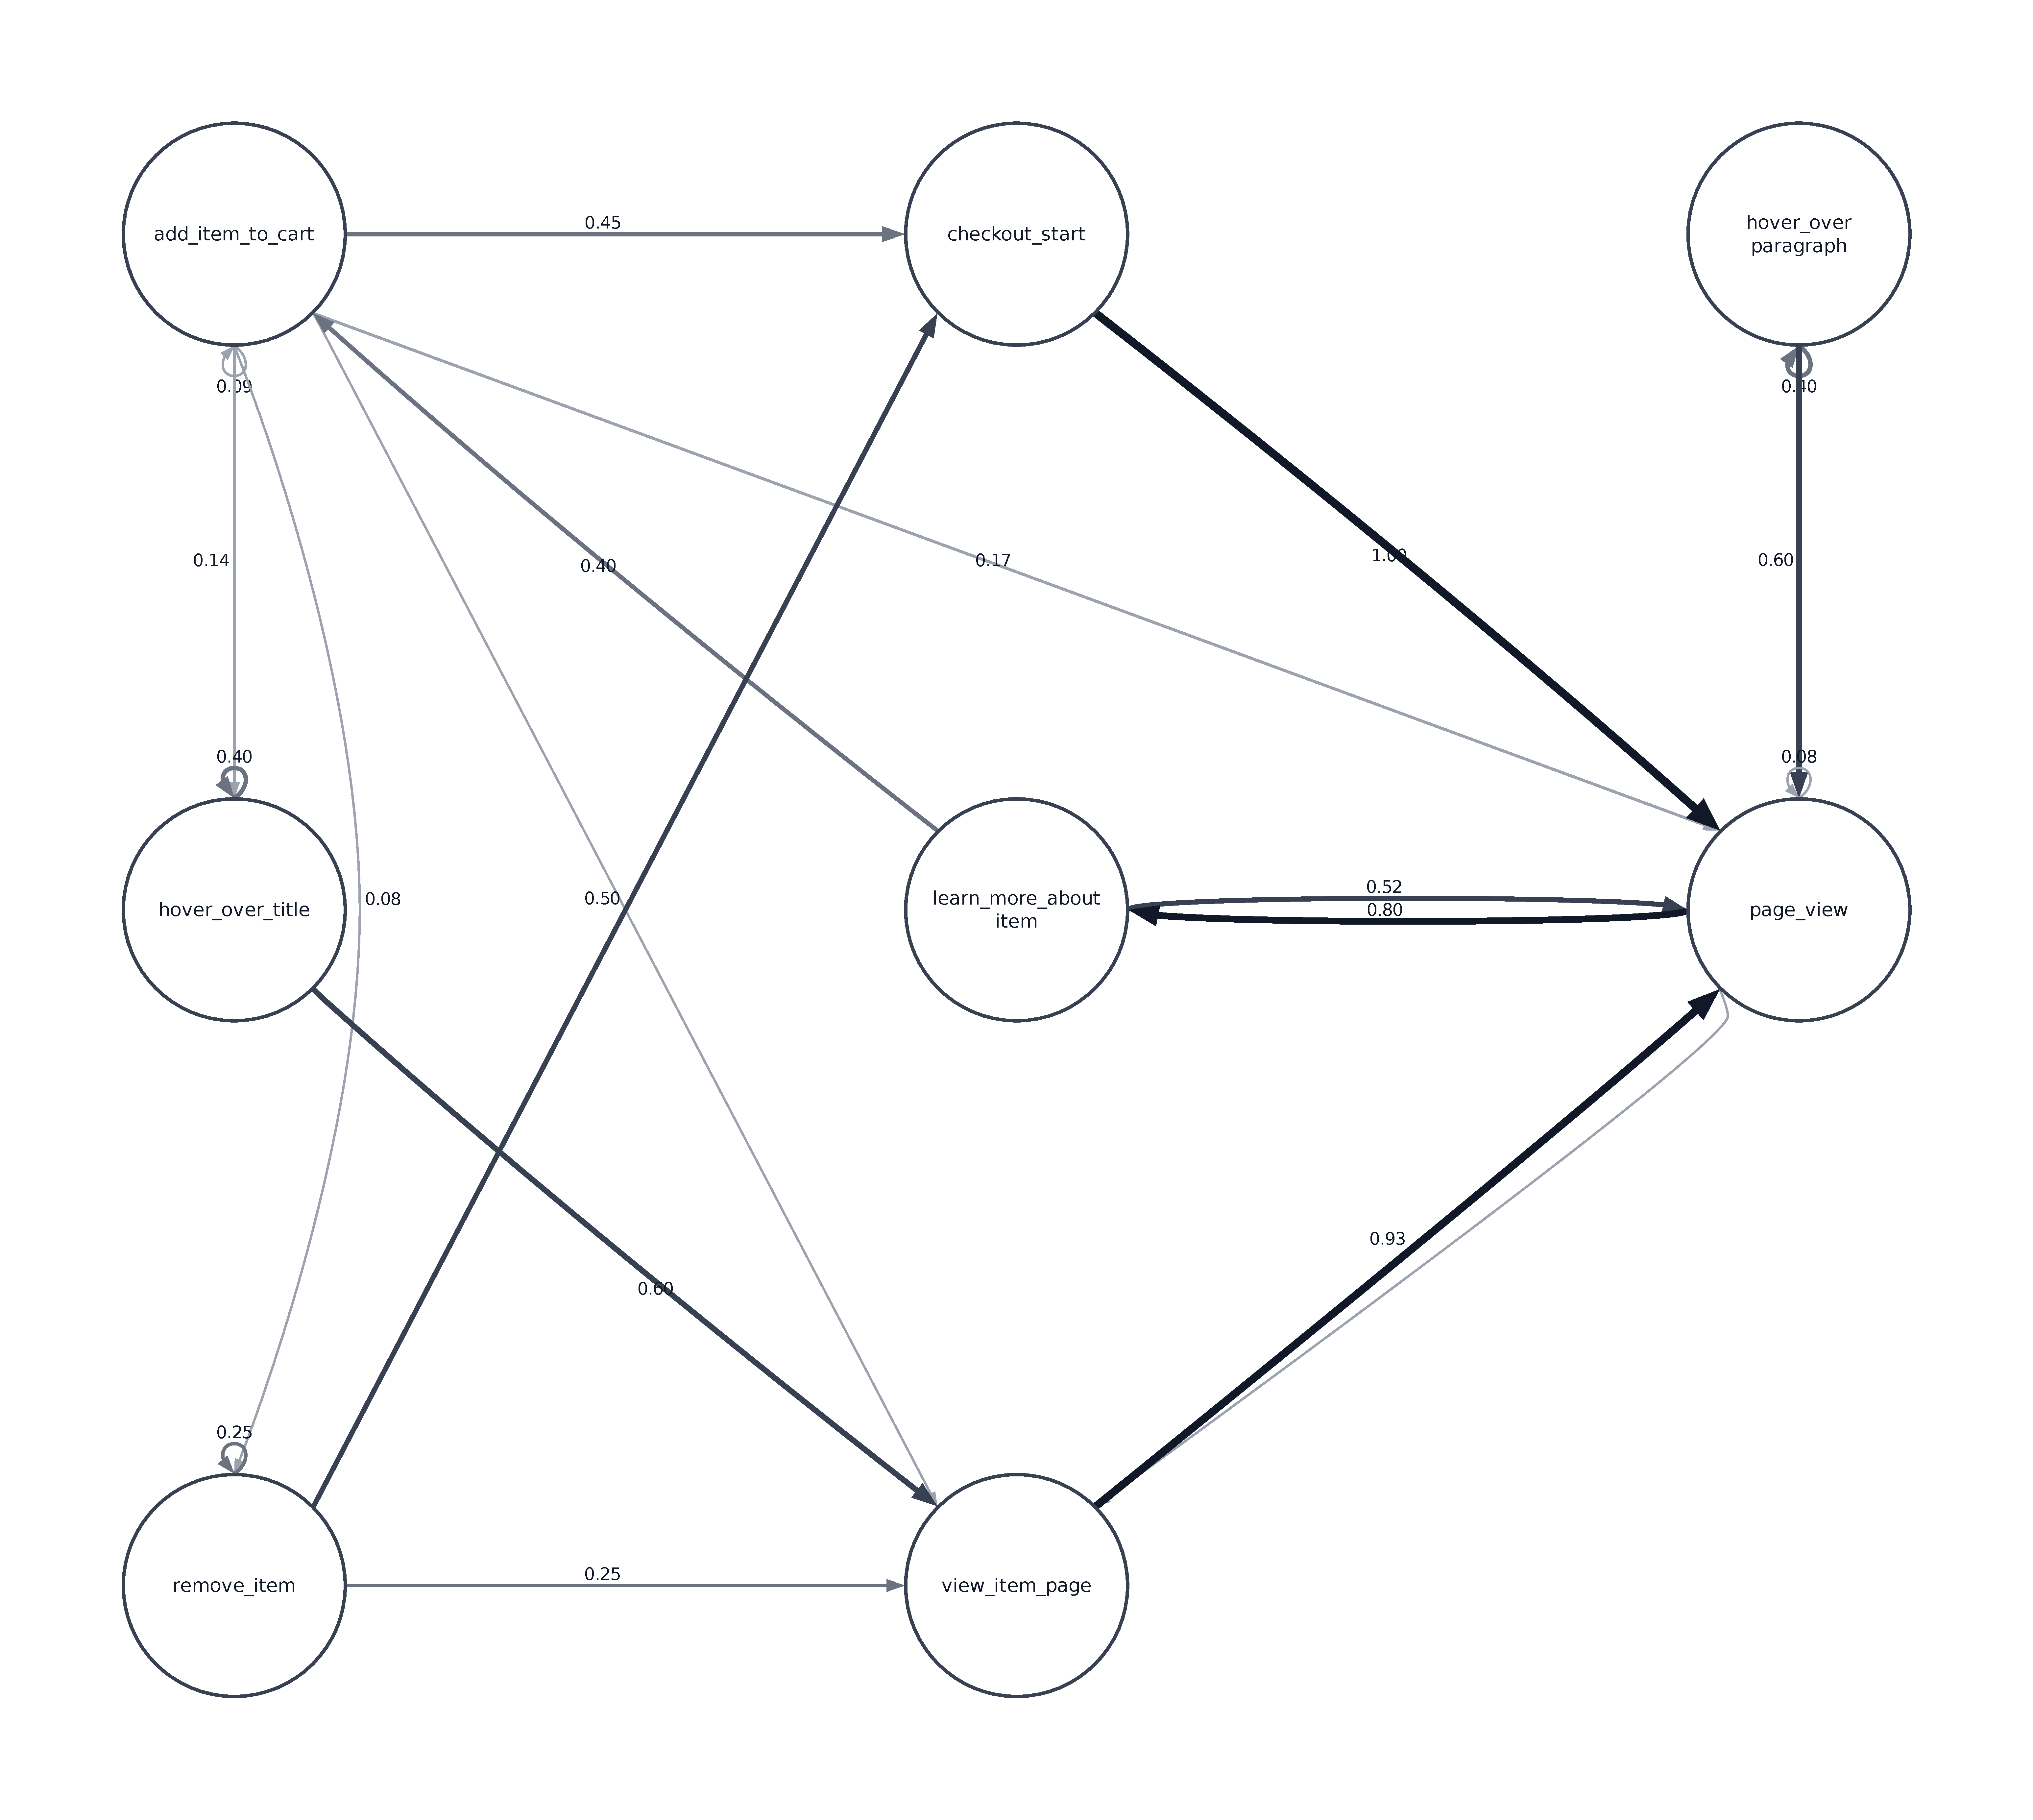
\includegraphics[width=0.8\textwidth]{chapters/mdp_human.pdf}
    \caption{Markov Decision Process visualization illustrating the behavioral transition dynamics for \textbf{human} actions.}
    \label{fig:human_mdp_viz}
\end{figure}

\begin{figure}[ht]
    \centering
    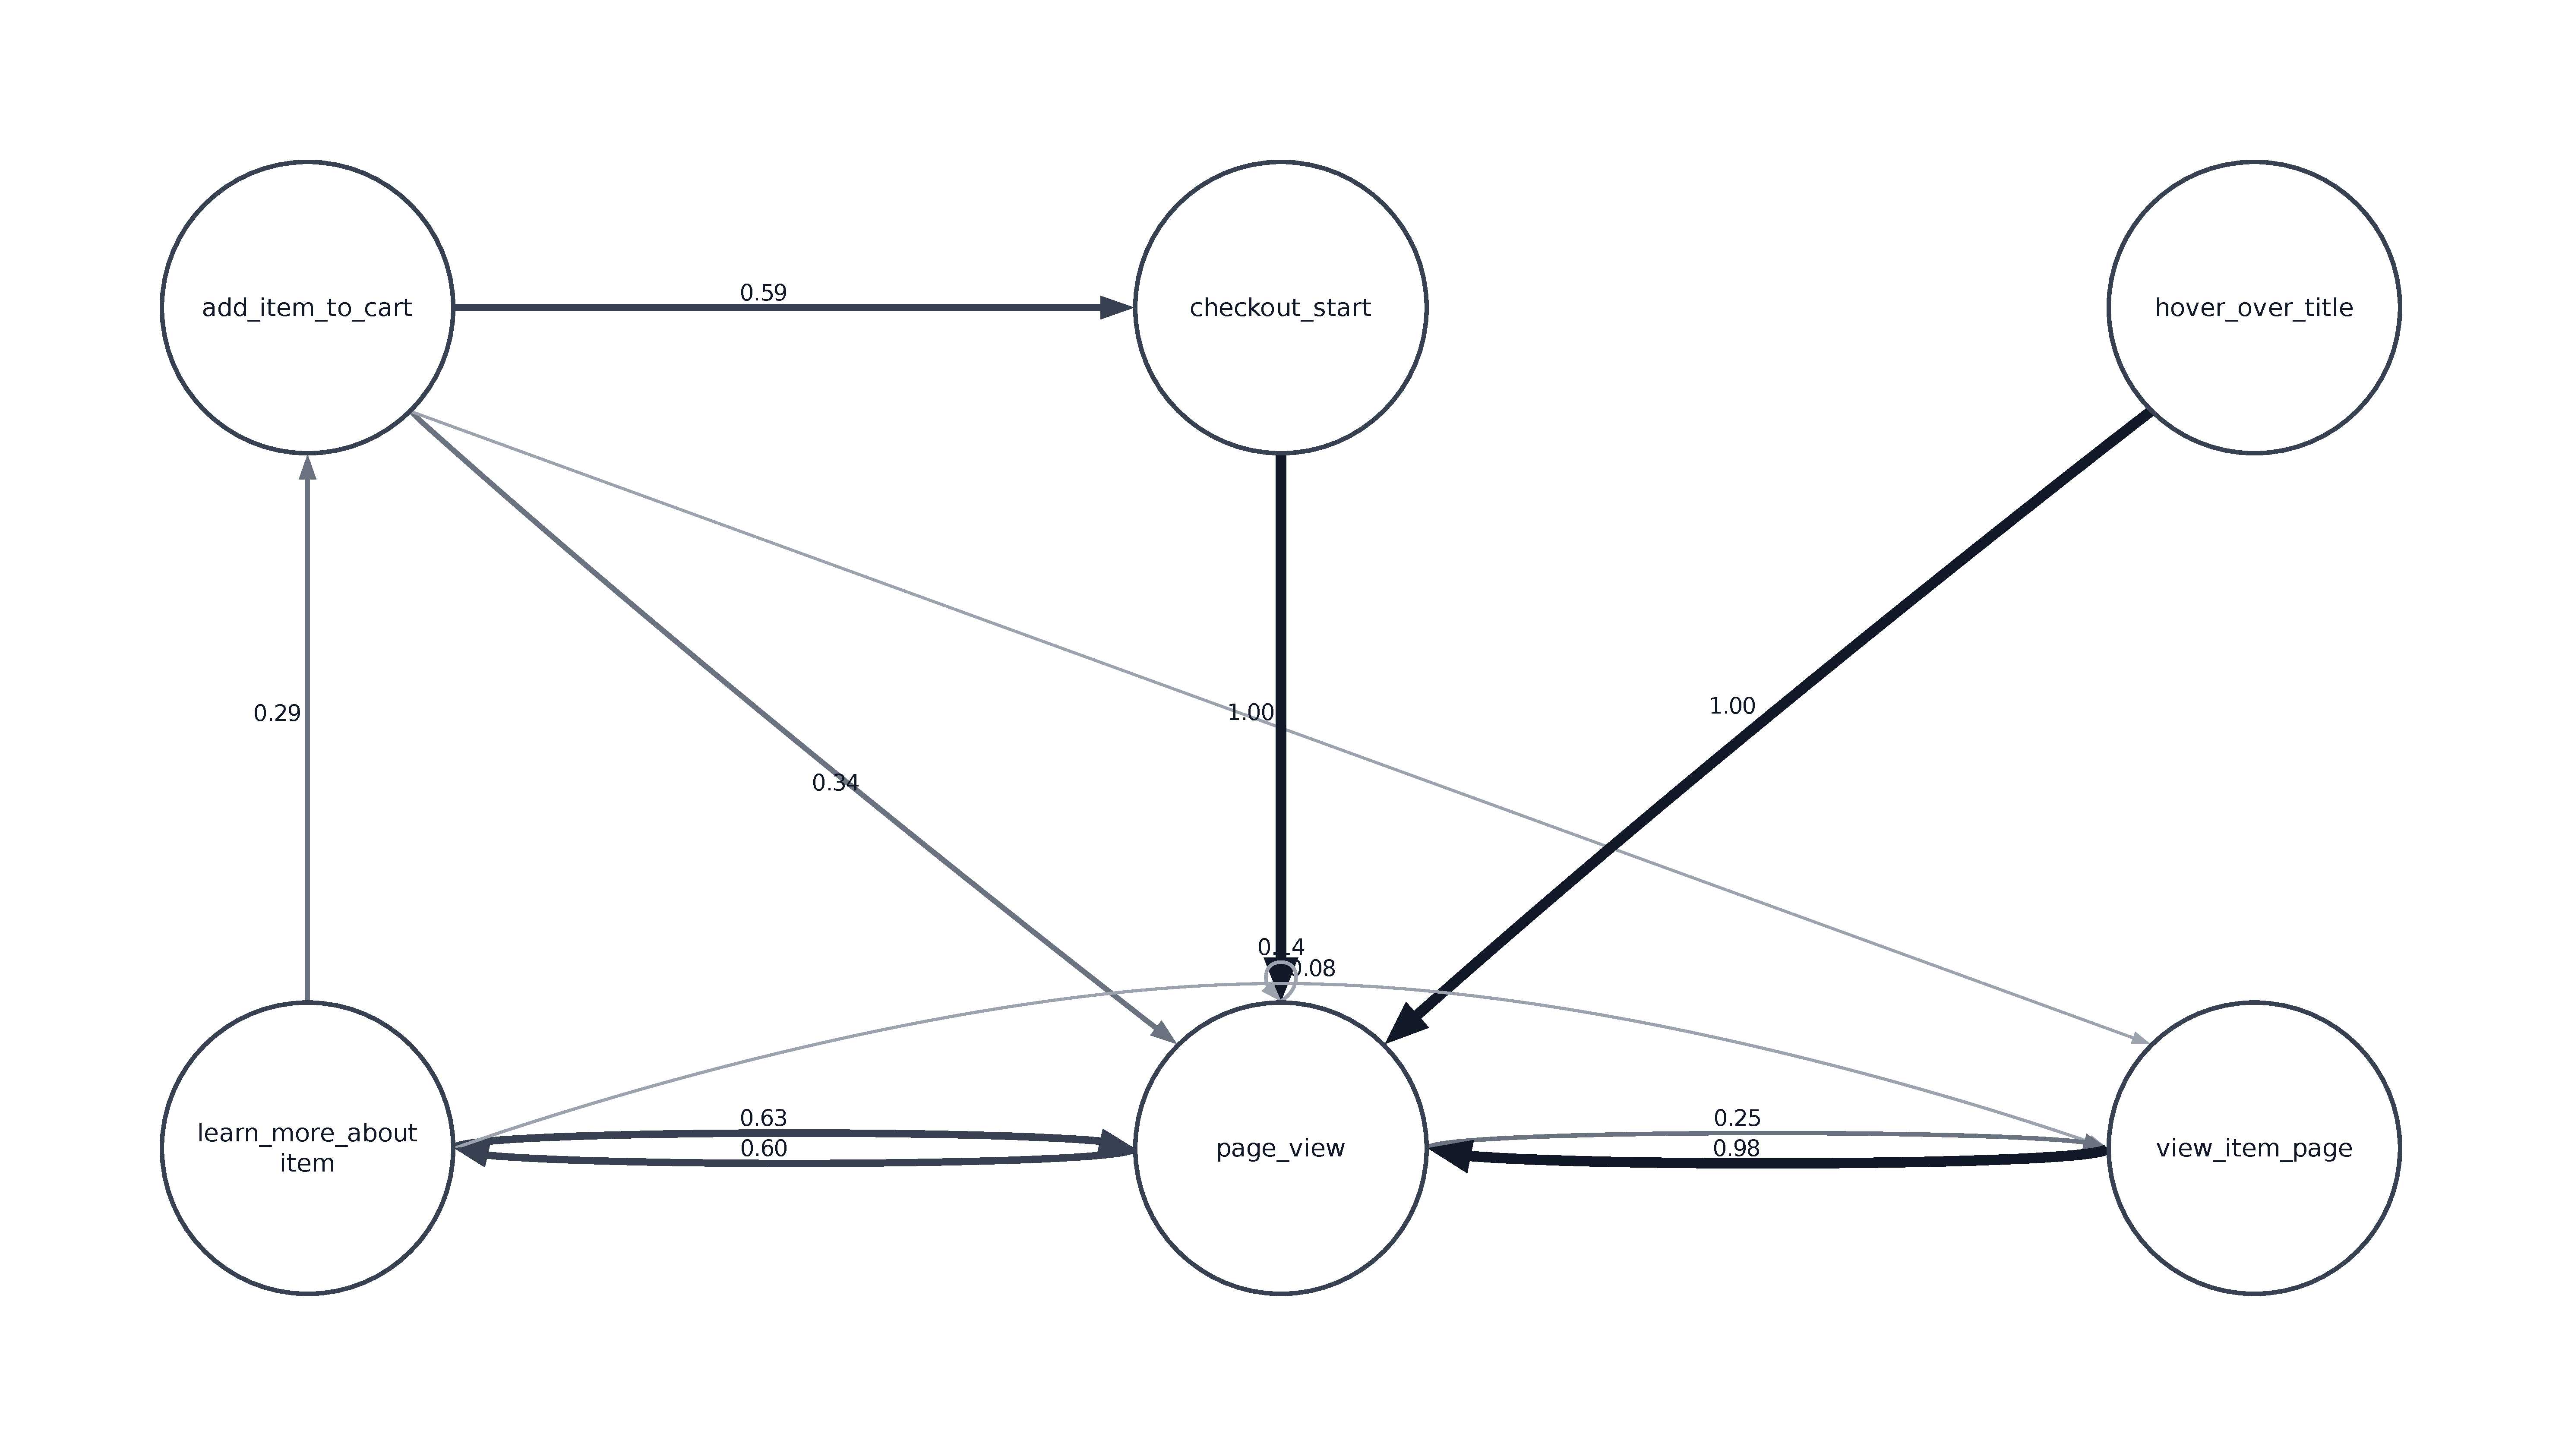
\includegraphics[width=0.8\textwidth]{chapters/mdp_agent.pdf}
    \caption{Markov Decision Process visualization illustrating the behavioral transition dynamics for \textbf{agent} behavior profiles. The state space and transition probabilities are learned from observed session trajectories to enable generative contamination.}
    \label{fig:agent_mdp_viz}
  \end{figure}

\subsection{Distributionally Robust Reinforcement Learning (DR-RL)}

We formulate pricing as a Stackelberg game: the platform (leader) sets prices, and the population (follower) responds through trajectories and demand. A useful intuition is that the platform behaves like a distorted mirror at a 45-degree angle: what it mirrors is population demand into an estimated demand proxy, and that proxy drives revenue.

Because contamination level and demand shift are non-stationary online, a simple error term is not enough. We therefore use a Distributionally Robust Optimization objective. For each newly observed trajectory generated by an unknown actor profile, we need a demand mapping conditioned on price and trajectory. For each trajectory, we compute its transition kernel and compare it with controlled baselines for humans and agents.

We compute two divergence scores: divergence from the human baseline and divergence from the agent baseline. This yields two centroid-like heuristics that act as a session-level agent score in the engine. On a per-customer or use-case basis a similar study should be done in order to obtain ground truth behavior models for humans and agents and their specific interaction with a given products website.

In implementation, we maintain an alternating game-history stack (our Limbo stack) and execute it explicitly every epoch with exactly two transitions: first the platform publishes a price vector (leader move), then the market responds with trajectory-derived demand (follower move).

\subsubsection{Ambiguity Set Construction}

We define an ambiguity set centered around our empirical reference distribution (derived from the generator). We utilize a distance metric to define the set of plausible demand distributions the agent might face: the ambiguity set contains all distributions that are statistically close to our observed training data but allows for adversarial shifts.

For the current engine baseline, we use a compact approximation by applying ambiguity over contamination in a local interval around nominal contamination: we consider all contamination values within a small radius of the target contamination level, and we evaluate a small fixed grid in that interval per step, selecting the worst-case candidate for the learner.

\subsubsection{Environment Setup for Dynamic Pricing}

The complete pricing-demand-trajectory loop is illustrated in the oracle flow figure. The Oracle maps historical price and demand state to a new price vector, which is exposed to a distribution of demand curves. Each product generates trajectories weighted by behavioral kernels, producing a full transition matrix over sessions. Sampled trajectories are aggregated through the demand proxy function to yield the next demand vector, which feeds back into the Oracle.

\begin{figure}[ht]
\centering
The oracle takes previous prices and demand, outputs new prices for each product. Each product's price generates demand curves from a distribution. Demand curves are combined with behavioral transition patterns to create a full transition matrix. We sample trajectories from this matrix, aggregate them through the demand proxy function, and get the next demand vector, which feeds back into the oracle.
\caption{Oracle-based pricing loop: historical price and demand state map to a new price vector; each product samples demand curves; trajectories are generated by mixing demand with behavioral kernels into transition matrix; sampled trajectories aggregate through proxy to yield updated demand, closing the feedback loop.}
\label{fig:oracle_flow}
\end{figure}

\subsubsection{The Min-Max Objective}

The robust policy is obtained by solving the maximin problem: we want to maximize revenue in the worst-case scenario. Specifically, we choose a pricing policy that maximizes the minimum expected reward across all plausible demand distributions in the ambiguity set. The reward consists of revenue from sales minus a penalty for information leakage.

In practice, we parameterize this with a session-level leakage term: information leakage equals the agent probability (how likely this session is from an agent) multiplied by the information value of the price quote. For the baseline engine, we use a constant query-tax surrogate: each suspected agent query incurs a fixed leakage cost.

Another possible extension is to adapt the ambiguity radius online based on observed divergence, so the uncertainty set changes with live data. We keep this as future work and retain a fixed-radius setup.

\subsubsection{Actor Implementation}

In our simulation, the follower is implemented as a set of Actors. Each Actor is initialized with a type which samples a specific demand curve from the latent distribution. This formalization ensures that our agent does not overfit to a single deterministic demand function but learns a policy robust to the distributional uncertainty.

Practical implementation of browser agents is a strongly evolving field with near-weekly releases of state-of-the-art architectures. In this thesis implementation we abstract that layer into trajectory generators learned from observed human/agent transition kernels.

As part of reward engineering, we keep a UX factor (user experience, ranging from 0 to 1) as an auxiliary evaluation axis. In the current baseline it is not injected into the core reward; it is tracked separately to compare policy trade-offs.

\begin{figure}[ht]
  \centering
  \resizebox{0.5\columnwidth}{!}{%
    
\begin{tikzpicture}[
    % Styles for consistency
    axis/.style={->, >=Stealth, line width=1.2pt, color=black!85},
    curve/.style={color=black, line width=2.5pt},
    point/.style={circle, fill=black, inner sep=0pt, minimum size=6pt},
    label_text/.style={font=\large, align=center, color=black},
    annotation_line/.style={thick, -, color=black!60}
]

    % Define Radius
    \def\R{5}

    % Draw Axes
    % Extended slightly beyond radius (\R + 1)
    \draw[axis] (0,0) -- (\R+1.5,0) node[midway, below=10pt, font=\bfseries\large] {UX Index};
    \draw[axis] (0,0) -- (0,\R+1.5) node[midway, left=15pt, rotate=90, font=\bfseries\large] {Performance};

    % Draw Perfect 1/4 Circle
    % Syntax: arc (start_angle : end_angle : radius)
    \draw[curve] (0,\R) arc (90:0:\R);

    % 1. Paranoid (High Performance side) -> Angle 67.5 degrees
    \node[point] (p1) at (75:\R) {};
    \node[label_text, above right=0.1cm and 0.1cm of p1] (l1) {Paranoid};
    \draw[annotation_line] (l1) -- (p1);

    % 2. Perfect Detection (Exact Middle) -> Angle 45 degrees
    \node[point] (p2) at (45:\R) {};
    \node[label_text, above right=0.2cm and 0.2cm of p2] (l2) {Perfect Detection};
    \draw[annotation_line] (l2) -- (p2);

    % 3. No Detection (High UX side) -> Angle 22.5 degrees
    \node[point] (p3) at (15:\R) {};
    \node[label_text, right=0.5cm of p3] (l3) {No Detection};
    \draw[annotation_line] (l3) -- (p3);

\end{tikzpicture}

  }
  \caption{Introducing the UX index allows us to better distinguish the kind of impact different methods have and allows us to compare them on this Pareto-like scale.}
\end{figure}

We also consider taxation-like overlays for agent traffic under strategy-proof mechanism design (e.g., Vickrey-Clarke-Groves style rules). This remains an extension path and is not part of the main implementation in this thesis.

\subsubsection{Pricing Mechanism Summary}

We now present the complete pricing mechanism that integrates the behavioral distinguishability, contamination estimation, and robust optimization components developed in the preceding sections. The defensive pricing loop algorithm formalizes the process as a Stackelberg game where the platform (leader) sets prices and the aggregate demand (follower) responds through observed session trajectories.

\begin{algorithm}[t]
\caption{PHANTOM defensive pricing loop}
\label{alg:phantom_loop_clean}
\DontPrintSemicolon
\SetKwInput{Input}{Input}
\SetKwInput{Output}{Output}

\Input{catalog size N; action scale grid; nominal contamination; ambiguity radius; candidate count K; horizon T; sessions per step M; behavior kernels for humans and agents; event weights; COI penalty}
\Output{trajectory of price, demand, and contamination over time}

\For{each time step t from 0 to T-1}{
  observe previous demand and price\;
  choose discrete action from policy\;
  set new price by scaling previous price with chosen action, keeping within bounds\;

  define local ambiguity interval around nominal contamination\;
  \For{each candidate k from 1 to K}{
    set contamination level for this candidate from a uniform grid\;
    sample M sessions from mixture of human and agent behaviors weighted by contamination\;
    compute demand proxy by summing weighted actions across all sessions\;
    compute divergence scores and session agent score from transition kernel\;
    compute candidate reward as revenue minus COI leakage penalty\;
  }
  choose worst-case candidate (lowest reward), set contamination to that level\;
  set demand and reward to worst-case values\;
}
\end{algorithm}

The algorithm operates in discrete epochs indexed by time. At each epoch, the platform applies one discrete multiplicative price action, the environment samples a batch of sessions, and demand is recomputed from weighted events. Robustness is implemented as an inner minimization over a small local grid of contamination candidates around nominal contamination, matching the current engine implementation. The history buffer enforces the alternating Stackelberg structure by preserving the temporal sequence of price publications and demand observations.
